\documentclass[12pt]{article}
\usepackage[hidelinks]{hyperref}    % permette di usare references cliccabili
\usepackage[all]{hypcap}    % porta sopra l'immagine dopo le references invece della caption di queste
\usepackage{graphicx}   % permette di inserire immagini
\usepackage{circuitikz} % permette di inserire porte logiche 
\graphicspath{{../images/}} % imposta path per trovare le immagini, i .. significano "la dir precedente"
\author{Andrea Malvezzi}
\title{\textbf{Architettura degli Elaboratori~-~Introduzione}}  % textbf = testo bold
\date{19 Settembre, 2024}
\begin{document}
\maketitle  % inserisce il titolo specificato in precedenza
\pagebreak
\section*{A cosa serve questo corso?}   % section* = non numerata, section = numerata
L'architettura degli elaboratori cerca di spiegare il funzionamento dei calcolatori dal punto di vista dell'hardware \textit{(HW)}.
\section {La composizione dei calcolatori}
\subsection{Le porte logiche}
Un calcolatore è composto da migliaia di componenti, tra cui le \textbf{PORTE LOGICHE}.\\
Esistono diversi tipi di porte logiche, ma due di queste~-~la NAND e la NOR~-~nutrono di una peculiarità: queste sono dette "\textbf{UNIVERSALI}" in quanto combinandole tra loro è possibile produrre tutte le altre funzioni logiche (o \textit{booleane}).
\subsection{In dettaglio}
\subsubsection{Porta logica AND}
\begin{circuitikz} \draw(0, 2) node[and port, number inputs=2](myand){} % draw(x, y)
    (myand.in 1) node[anchor=east]{A}
    (myand.in 2) node[anchor=east]{B}
    (myand.out) node[anchor=west]{Output}
    ;
\end{circuitikz}
\hfill
\begin{tabular}{|| c c c ||}
    \hline
    A & B & Output\\
    \hline
    0 & 0 & 0\\
    \hline
    0 & 1 & 0\\
    \hline
    1 & 0 & 0\\
    \hline
    1 & 1 & 1\\
    \hline
\end{tabular}\\\\
La funzione logica AND restituisce VERO (\textit{1}) soltanto quando entrambi i valori in ingresso sono VERO.\\
Nell'algebra booleana si indica con il simbolo della moltiplicazione "$\times$", o scrivendo vicini due valori (come (a)(b) equivale ad a$\times$b).
\pagebreak
\subsubsection{Porta logica OR}
\begin{circuitikz} \draw(0, 2) node[or port, number inputs=2](myor){}
    (myor.in 1) node[anchor=east]{A}
    (myor.in 2) node[anchor=east]{B}
    (myor.out) node[anchor=west]{Output}
    ;
\end{circuitikz}
\hfill
\begin{tabular}{|| c c c ||}
    \hline
    A & B & Output\\
    \hline
    0 & 0 & 0\\
    \hline
    0 & 1 & 1\\
    \hline
    1 & 0 & 1\\
    \hline
    1 & 1 & 1\\
    \hline
\end{tabular}\\\\
La funzione logica OR restituisce VERO quando \underline{almeno} uno dei due valori in ingresso è VERO.\\
Nell'algebra booleana si indica con il simbolo della somma (+).
\subsubsection{Porta loica XOR}
\begin{circuitikz} \draw(0, 2) node[xor port, number inputs=2](myxor){}
    (myxor.in 1) node[anchor=east]{A}
    (myxor.in 2) node[anchor=east]{B}
    (myxor.out) node[anchor=west]{Output}
    ;
\end{circuitikz}
\hfill
\begin{tabular}{|| c c c ||}
    \hline
    A & B & Output\\
    \hline
    0 & 0 & 0\\
    \hline
    0 & 1 & 1\\
    \hline
    1 & 0 & 1\\
    \hline
    1 & 1 & 0\\
    \hline
\end{tabular}\\\\
La funzione logica XOR restituisce VERO quando \underline{soltanto} uno dei due valori in ingresso è VERO.\\
Nell'algebra booleana si indica con il simbolo "$\oplus$".
\subsubsection{Porta logica NOT}
\begin{circuitikz} \draw(0,1) node[not port, number inputs=1](mynot){}
    (mynot.in 1) node[anchor=east]{A}
    (mynot.out) node[anchor=west]{Output}
    ;
\end{circuitikz}
\hfill
\begin{tabular}{||c c||}
    \hline
    A & Output\\
    \hline
    0 & 1\\
    \hline
    1 & 0\\
    \hline
\end{tabular}\\\\
La funzione logica NOT "nega" effettivamente il valore entrante, invertendolo. Quindi da un valore vero se ne otterrà uno falso e viceversa.\\
Quando collocata in seguito ad altre porte logiche si indica con un piccolo cerchio.
\subsubsection{Porta logica NAND}
\begin{circuitikz} \draw(0, 2) node[nand port, number inputs=2](mynand){}
    (mynand.in 1) node[anchor=east]{A}
    (mynand.in 2) node[anchor=east]{B}
    (mynand.out) node[anchor=west]{Output}
    ;
\end{circuitikz}
\hfill
\begin{tabular}{||c c c||}
    \hline
    A & B & Output\\
    \hline
    0 & 0 & 1\\
    \hline
    0 & 1 & 1\\
    \hline
    1 & 0 & 1\\
    \hline
    1 & 1 & 0\\
    \hline
\end{tabular}\\\\
La funzione logica NAND è la porta AND seguita da una NOT, quindi basta invertire i risultati della sua tabella di verità.
\subsubsection{Porta logica NOR}
\begin{circuitikz} \draw(0, 2) node[nor port, number inputs=2](mynor){}
    (mynor.in 1) node[anchor=east]{A}
    (mynor.in 2) node[anchor=east]{B}
    (mynor.out) node[anchor=west]{Output}
    ;
\end{circuitikz}
\hfill
\begin{tabular}{||c c c||}
    \hline
    A & B & Output\\
    \hline
    0 & 0 & 1\\
    \hline
    0 & 1 & 0\\
    \hline
    1 & 0 & 0\\
    \hline
    1 & 1 & 0\\
    \hline
\end{tabular}\\\\
La funzione logica NOR, come la NAND, altro non è che una porta OR seguita da una NOT. Quindi basterà invertire i valori di verità della funzione logica OR per ottenere quelli della sua controparte negata.
\subsubsection{La funzione logica OR con la porta NAND}
\begin{circuitikz} \draw
    (0, 2) node[nand port, number inputs=2](topnand){}
    (topnand.in 1) node[anchor=east]{A}
    (topnand.in 2) node[anchor=east]{B}
    (0, 0) node[nand port, number inputs=2](botnand){}
    (botnand.in 1) node[anchor=east]{A}
    (botnand.in 2) node[anchor=east]{B}
    (2, 1) node[nand port, number inputs=2](nextnand){}
    (nextnand.out) node[anchor=west]{Output}
    (topnand.out) -- (nextnand.in 1)
    (botnand.out) -- (nextnand.in 2)
    ;
\end{circuitikz}\\
Per verificare la correttezza del circuito, inserire i valori di verità desiderati e paragonare l'output con quello della tabella di verità della porta OR.
\pagebreak
\subsubsection{La funzione logica AND con la porta NAND}
\begin{circuitikz} \draw
    (0, 2) node[nand port, number inputs=2](firstnand){}
    (firstnand.in 1) node[anchor=east]{A}
    (firstnand.in 2) node[anchor=east]{B}
    (2, 2) node[nand port, number inputs=2](secondnand){}
    (secondnand.out) node[anchor=west]{Output}
    (firstnand.out) -- (secondnand.in 1)
    (firstnand.out) -- (secondnand.in 2)
    ;
\end{circuitikz}\\
Per verificare la correttezza del circuito, inserire i valori di verità desiderati e paragonare l'output con quello della tabella di verità della porta AND.
\pagebreak
\subsection{Il principio di Astrazione/Implementazione}
Per realizzare sistemi complessi partendo da queste porte si usa il \textbf{principio di "Astrazione/Implementazione"}:
\begin{itemize} % lista disordinata
    \item Astrazione: si frammenta il problema di partenza in problemi minori, più semplici da risolvere.
    \item Implementazione: si realizza la soluzione al problema di partenza combinando tra loro le soluzioni minori precedentemente escogitate.
\end{itemize}
\section{Elaboratori multilivello}
Un elaboratore può essere composto da più livelli e generalmente è corretto dire che i livelli superiori sono destinati alla rsoluzione di problemi mediante linguaggi adatti, mentre quelli inferiori sono improntati alla gestione delle risorse e alla comunicazione tra HW e SW.\\
\begin{figure}[!htb]
    \centering
    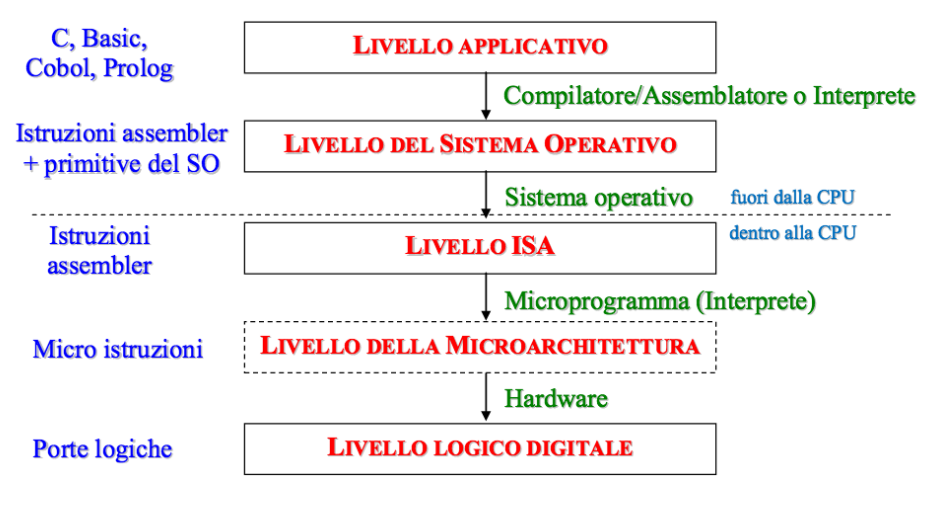
\includegraphics[width=.9\linewidth,height=.40\textheight,keepaspectratio]{introduzione/struttura_multilivello.PNG} % essenzialmente resiza l'immagine
    \begin{center}
        \caption{\label{fig:multilevel_example}Un esempio della struttura di un elaboratore a più livelli.} % label fuori da caption spesso non va, mettilo dentro
    \end{center}
\end{figure}
\subsection{Livello 0: livello logico digitale}
Qui si hanno le porte logiche e conseguentemente è dove avvengono le relative operazioni.
\subsection{Livello 1: livello di microarchitettura}
La microarchitettura è ciò che in un elaboratore gestisce il flusso di dati tra i vari componenti.\\
Può trattarsi sia di HW che di SW.
\subsection{Livello 2: livello ISA(Instruction Set Architecture)}
Funge da interfaccia da HW e SW.\\
Contiene le istruzioni che vengono eseguite nella microarchitettura.
\subsection{Livello 3-4: O.S. e Assembly}
Qui si programmano i livelli sottostanti, si gestiscono le risorse del sistema e si eseguono i programmi.
\subsection{Livello 5: livello del linguaggio}
Qui è dove si usano linguaggi più vicini agli esseri umani per risolvere problemi e fornire servizi. Il codice di questi linguaggi dovrà essere tradotto in linguaggio macchina per essere eseguito.\\
Vedi "Livello applicativo" nell'immagine~\ref{fig:multilevel_example}.
\end{document}